\subsection{Информационная модель системы}
\label{sec:develop:erDiagrams}

Чтобы разработать мобильное приложение для управления адресной светодиодной лентой необходимо представить информационную модель этой системы. Система рассмотрена в виде совокупности объектов и связей между ними. 

Представления информационной модели в графическом виде (логический и физический уровни) приведены на рисунках \ref{fig:develop:erDiagrams:erLogic} и \ref{fig:develop:erDiagrams:erPhysic}.

Нормальная форма — требование, предъявляемое к структуре таблиц в теории реляционных баз данных для устранения из базы избыточных функциональных зависимостей между атрибутами (полями таблиц).

Отношение находится в первой нормальной форме, если все его атрибуты являются простыми, все используемые домены должны содержать только скалярные значения.

Отношение находится во второй нормальной форме, если оно находится в первой нормальной форме и каждый не ключевой атрибут неприводимо зависит от Первичного Ключа.

Отношение находится в третьей нормальной форме, когда находится во второй нормальной форме и каждый не ключевой атрибут нетранзитивно зависит от первичного ключа. Проще говоря, второе правило требует выносить все не ключевые поля, содержимое которых может относиться к нескольким записям таблицы в отдельные таблицы \cite{er_info}.

Исходя из данной информации, модель, представленная в данной главе находится в третьей нормальной форме.

~
\begin{figure}[H]
\centering
	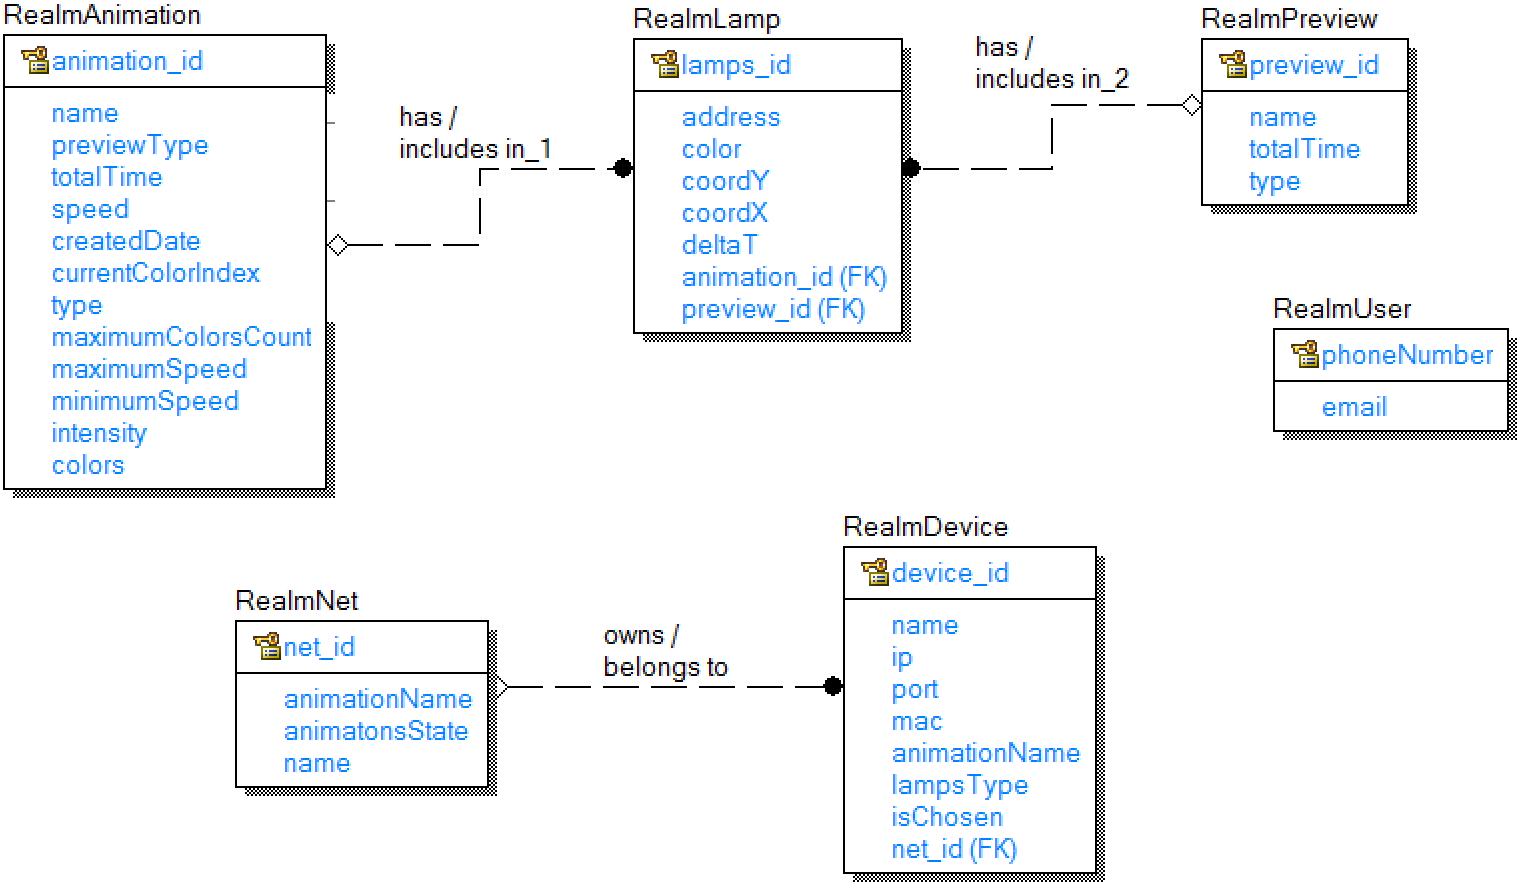
\includegraphics[scale=0.6]{figures/diagrams/er_diagram_logic.png}
	\caption{Логический уровень информационной модели приведенной к третьей нормальной форме}
	\label{fig:develop:erDiagrams:erLogic}
\end{figure}

~
\begin{figure}[H]
\centering
	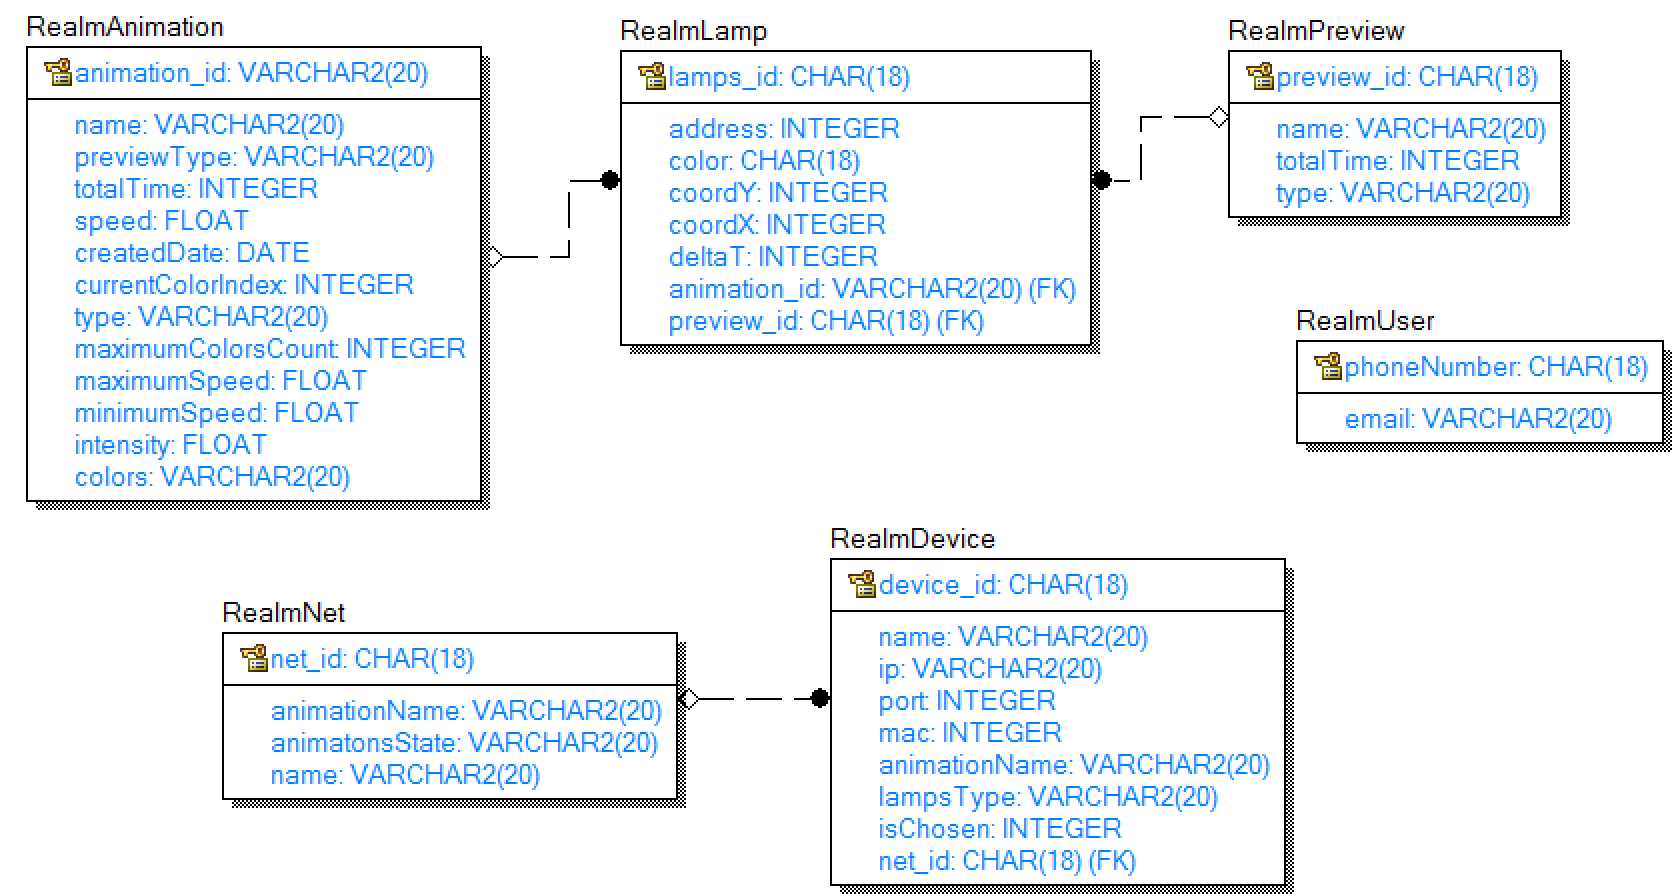
\includegraphics[scale=0.55]{figures/diagrams/er_diagram_physical.png}
	\caption{Физический уровень информационной модели приведенной к третьей нормальной форме}
	\label{fig:develop:erDiagrams:erPhysic}
\end{figure}

При проектировании системы для управления адресной светодиодной лентой были выделены такие сущности, как:
\begin{itemize}
	\item Анимация;
	\item Лампочка;
	\item Отображение;
	\item Сеть;
	\item Устройство (адресная светодиодная лента);
	\item Пользователь.
\end{itemize}

Сущность Анимация необходима для отображения стандартных и пользовательских анимаций в приложении и содержит в себе следующие атрибуты:
\begin{itemize}
	\item name~-- имя анимации;
	\item animation\_id~-- id анимации, используется при отправке анимации на адресную светодиодную ленту (0~-- посылается через байты, 1, 2,...~-- запускает анимацию внутри самой адресной ленты);
	\item previewType~-- тип анимации (default, custom);
	\item totalTime~-- полное время анимации;
	\item speed~-- скорость анимации;
	\item type~-- тип отображения в приложении (string, tree, custom, grid);
	\item createdDate~-- дата создания;
	\item currentColorIndex~-- выбранный набор цветов;
	\item maximumColorsCount~-- максимальное количество цветов в наборе;
	\item maximumSpeed~-- максимальное значение скорости;
	\item minimumSpeed~-- минимальное значение скорости;
	\item intensity~-- интенсивность анимации;
	\item editOptions~-- доступные опции для редактирования;
	\item colors~-- наборы цветов.
\end{itemize}

Сущность Лампочка необходима для представления лампочки на адресной светодиодной ленте под определенным адресом в конкретный момент времени и содержит в себе следующие атрибуты:
\begin{itemize}
	\item lamps\_id~-- id лампочки;
	\item address~-- адрес лампочки;
	\item color~-- цвет лампы;
	\item coordX~-- координата по оси абсцисс;
	\item coordY~-- координата по оси ординат;
	\item deltaT~-- момент времени, когда лампочка должна загореться;
	\item animation\_id~-- id анимации, к которой принадлежит лампочка;
	\item preview\_id~-- id отображения, к которому принадлежит лампочка.
\end{itemize}

Сущность Отображение необходима для представления адресной светодиодной ленты на экране приложения и содержит в себе следующие атрибуты:
\begin{itemize}
	\item preview\_id~-- id отображения;
	\item name~-- имя отображения;
	\item totalTime;
	\item type~-- тип отображения;
	\item lamps~-- лампочки отображения.
\end{itemize}

Сущность Сеть необходима для представления сети из адресных светодиодных лент и содержит в себе следующие атрибуты:
\begin{itemize}
	\item net\_id~-- id сети;
	\item name~-- имя сети;
	\item animationName~-- имя анимации, проигрываемой на сети;
	\item animationState~-- тип отображения анимаций в сети;
	\item devices~-- устройства в сети.
\end{itemize}

Сущность Устройство необходима для представления адресной светодиодной ленты в сети и содержит в себе следующие атрибуты:
\begin{itemize}
	\item device\_id~-- id устройства;
	\item name~-- имя устройства;
	\item ip~-- ip-адрес устройства;
	\item port~-- порт в сети;
	\item mac~-- mac-адрес устройства;
	\item animationName~-- проигрываимая анимация на устройстве;
	\item lampsType~-- тип лампочек на устройстве;
	\item isChosen~-- флаг выбрано ли устройство для анимирования в сети;
	\item net\_id~-- id сети, к которому принадлежит устройство.
\end{itemize}

Сущность Пользователь необходима для представления пользователя для отправки анимаций и содержит в себе следующие атрибуты:
\begin{itemize}
	\item phoneNumber~-- номер телефона пользователя;
	\item email~-- email-адрес пользователя.
\end{itemize}